\chapter{Binary Instrumentation}
Binary instrumentation is the operation of inserting new code at any point into an existing binary to observe and
possibly modifiy its behaviour; the point at which the new code is added is the \textit{instrumentation point} while the
added instructions are the \textit{instrumentation code}. Binary instrumentation can also be used to improve the
resilience of a binary - e.g. insrumenting {\ttfamily call} and {\ttfamily ret} to ensure that the control flow is
redirected only to a list of expected targets. Instrumenting a binary is no easy task as the insertion of additional
code would normally break all of the references; that's the reason why APIs have been developed to allow the
installation of callbacks at the instrumentation points. Instrumentation tools can be distinguished into static and
dynamic and will be detailed in the following sections.



\section{Static Binary Instrumentation}
Static Binary Instrumentation (SBI hereafter) uses binary rewriting on disks - i.e. the files are actually modified on
disk. SBI tools include PEBIL and Dynisnt (which actually supports bothSBI and DBI). The challenge, as already
mentioned, is to rewrite code without breaking any reference; in order to do so there are two known appproaches:
\begin{itemize}
    \item The {\ttfamily INT3} approach;
    \item The \textit{trampoline} approach.
\end{itemize}


\subsection{The INT3 Approach}
Due to the impossibility to introduce new code without breaking the binary, the additional code must be stored into a
separate location such as a new section or shared library. A possibility would be to substitute the instruction at the
instrumentation point with a {\ttfamily jmp} to the instrumentation code (which must include the originally substituted
instruction in order to maintain consistency in the code). The problem is that if the instrumentation code changes the
content of the registers it will change the program behaviour; thus the SBI tools must save the register state and
restore it at the end of the instrumentation phase (unless registers are voluntarily changed). The problem with this
approach is that normally the {\ttfamily jmp} instruction requires 5 bytes; therefore it is impossible to instrument any
instruction with a length shorter than this without corrupting the following instructions. Furthermore the potentially
corrupted instruction cannot be rewritten into the instrumentation code as it might be the target of a branch
instruction.
\begin{figure}[!htbp]
    \begin{center}
        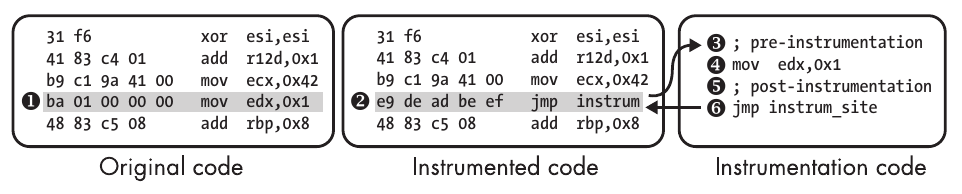
\includegraphics[scale=0.5]{./pics/naive_SBI.png}
        \caption{Naive SBI}
        \label{naive_SBI}
    \end{center}
\end{figure}
The {\ttfamily INT3} instruction, being only 1 byte long resolves the problem of multiple bytes instructions; {\ttfamily
INT3} generates a {\ttfamily SIGTRAP} which is caught by the SBI tool. At this point it becomes possible to use the
{\ttfamily PTRACE} set of functions to gain control of the flow and then execute the instrumented code.


\subsection{The Trampoline Approach}
The trampoline approach uses a completely different technique; the original code is copied and instrumented. In this
case references will not break as the instrumented code will be reached by means of  {\ttfamily jmp}s - i.e. the
\textit{trampolines}; whenever the control is transferred to the original code the trampolines will redirect it to the
corresponding instrumented chunks (which are located into the {\ttfamily .text.instrum}).
\begin{figure}[bpth]
    \begin{center}
        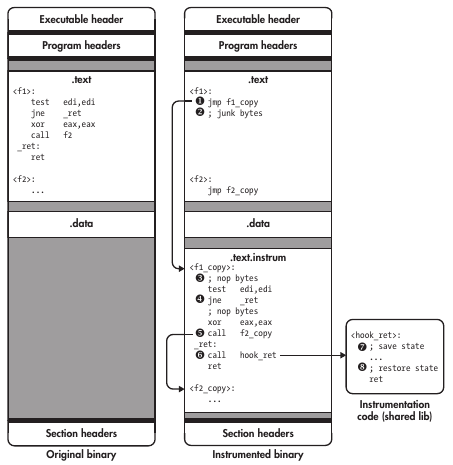
\includegraphics[scale=0.7]{./pics/trampoline.png}
        \caption{Trampoline}
        \label{trampoline}
    \end{center}
\end{figure}
As soon as a function is called the trampoline jumps to its copy; the jump instruction might corrupt the following ones,
but they are never executed in reality. The SBI inserts several {\ttfamily nop}s at the instrumentation points so that
the SBI can overwite them with a jump or a call. The insertion of the instrumentation code and {\ttfamily 0x90} is done
statically. Relative jumps are patched in order to maintain their correctness despite the code shifting caused by the
insertion of code; all of the 2 bytes long jumps, having an 8-bit offset, are replaced with 5 bytes long jumps, with a
32-bit offset, due to the fact that with the additional code 8 bits might not be enough to encode the jumps. The
{\ttfamily call} instructions are rewritten as to redirect the execution on the instrumented copy instead of the
original code. The instrumented code, which can be contained in a shared library, must save the state of the program at
the beginning of the instrumentation and restore it at the end.

\subsubsection{Indirect Control Flow}
Since indirect control flow target instructions at dynamically computed addresses they cannot be computed by the SBI;
this is managed by transferring control to the original code and using trampolines duly inserted in it. 
\paragraph{Indirect Calls} The SBI code does not alter the code that computes the addresses of indirect calls so that
indirect calls maintain the same functions as targets; these contain trampolines which hand the control over to
instrumented code.
\paragraph{Indirect Jumps} The situation is more complicated for indirect jumps; for example {\ttfamily switch}
statements are implemented through \textit{jump tables} containing all of the possible addresses of relevant {\ttfamily
case}'s. The indirect jump from one address to the other via the table lands in the original code; due to unexhaustive
basic symbolic information it is really difficult to patch the cases as there is no easy way to understand where the
trampolines are to be placed and there is also the underlying risk of corrupting them should there be not enough space
between one another. Patching the jump table is equally risky as it would be possible to change data that happens to be
a valid address instead.
\paragraph{Position-Indipendent Code} The analysis of PIE code requires special support as they might read the program
counter with instrumented code - i.e. with mutated references - and use it for address computations. In order to
overcome this pitfall SBI instruments the instruction reading the \reg{rip} as to let them return the result that they
would have in the original code.



\section{Dynamic Binary Instrumentation}
DBI monitors processes as they execute and instruments the instruction stream; no binary rewriting is needed and
therefore the technique is far less error prone. The DBI engines normally expose an API that allows for the selective
instrumentation of code. Before starting or attaching to the main application the DBI initialises itself by registering
functions for instrumentation. After initialisation the DBI engine is ready to start the application. DBI tools never
run processes directly, but run instruction in a code cache that contains the instrumented code. The code cache is
initially empty and the instrumentation engine fetches a chink of code - not necessarily a single block - from the
process and instruments it. After instrumentation the code is compiled with a JIT compiler and fed to the code cache for
execution. Control flow instructions are rewritten as to render control to the instrumentation engine, thus avoiding
control transfer to uninstrumented code. The JIT compiler does not translate the code into a different language, but
from native machine code to native machine code; it is only used to instrument the code and compile it the first time it
is executed. After that is cached and reused; the cached code is executed until there is a control flow instruction that
requires fetching another code chunk or block. Tools like DynamoRIO and Pin reduce the overhead by rewriting also these
control flow instructions and jumping directly to the next cached chunk; if this is not possible - i.e. indirect calls -
the rewritten instructions return control to the DBI engine that fectches the next code chunk. The instrumented code can
normally run natively, but some instructions need to be emulated - e.g. {\ttfamily syscalls} are handled in a particular
way by Pin. The instrumented code contains callbacks to functions in the DBI tool that observe or modify the code's
behaviour.
\begin{figure}[bpth]
    \begin{center}
        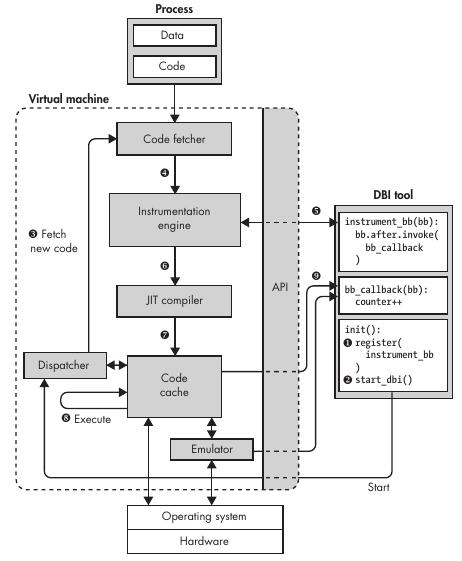
\includegraphics[scale=0.7]{./pics/DBI.png}
        \caption{DBI Architecture}
        \label{DBI}
    \end{center}
\end{figure}



\section{Hijacking the GOT/PLT}
Another way to instrument the code in PIE executables is hijacking the call to dynamic library functions by infecting
the GOT/PLT. The infection happens in two steps:
\begin{itemize}
    \item Hook injection;
    \item Patch the {\ttfamily GOT} and hijack call to redirect control flow on to the hook.
\end{itemize}
The drawback of these techniques is that exdcutables must be {\ttfamily PIC/PIE} and not use standard external
libraries. Figure \ref{LIEF} shows the inner workings of a cross platfrom tool called LIEF.

\begin{figure}[!bpth]
    \begin{center}
        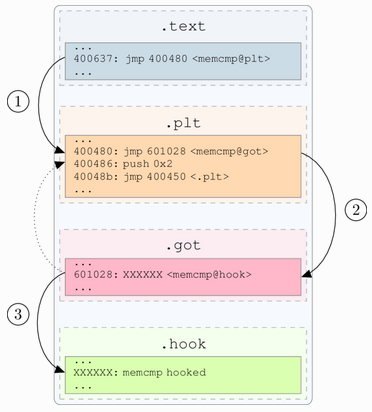
\includegraphics[scale=1.0]{./pics/lief.png}
        \caption{Library to Instrument Executable Formats}
        \label{LIEF}
    \end{center}
\end{figure}



\section{Transparency}
What explained so far introduced an important requirement for the development of instrumentation tools; these must avoid
interference with the normal execution flow unless necessary - i.e. they must be "transparent". Transparent design and
implementation of instrumentation tools has already been addressed in the previous chapters, but the concept will be
explored specifically in the present section. Most of the binaries execute introspective operations such as reading
registers and return addresses; if the instrumentation tools change the execution environment they might derail the
control flow in unuexpected ways or crash the process. This sparked the definition of the so called \textit{Transparency
Guidelines} which purpose is pushing developers to build efficient and successful instrumentation tools. These can be
summarised in three main points:
\begin{enumerate}
    \item Leave the application unchanged whenever possible;
    \item Changes shall be unperceivable from the application perspective;
    \item Avoid resource conflicts by requiring them directly from the OS and if using libraries fully isolate them from
        the application.
\end{enumerate}
These best practices translate in into specific requirements in the design and implementation of instrumentation tools.


\subsection{Transparency in System Design}

\subsubsection{Code Transparency}
Code transparency refers to the faithful reproduction of application behaviour with respect to changes in/to
references to its code when executing in an instrumentation/virtualisation system. This is normally achieved by using a
code cache which in reality complicates the transparency issues, but allows for great flexibility, effectiveness and
efficiency.
\paragraph{Address Transparency} Address transparency refers to the fact that every address manipulated by the
instrumentation must remain an original application address; thus indirect branch targets must be translated into cache
address and viceversa when a cache address is exposed to the original application control flow. The latter happens when
the OS passes the machine context or signal or exception handler; both the faulting or interrupted address must be made
available, along with the register state, as if the signal or exception happened natively and not in the instrumented
code.
\paragraph{Code Cache Consistency} The instrumentation tool must ensure that the code in the cache is consistent with
the original application code - e.g. unmapping a shared library from memory must result in flushing the cache of the
code contained in the associated region. The original code might also use self modifying instructions or reuse of the
memory region for dynamic code generation and in these cases the solution is to protect cache regions as read-only
areas; if an attempt to write is made the region is flushed, made writable and the faulting write is executed. A
complication with page protection occurs when an application requests output from a syscall at an address in the read
only region; in this case a possible solution could be to look for all of the input parameters, if known, in the read
only areas and swap those pages to use sandboxing.

\subsubsection{Data Transparency}
\paragraph{Application State Preservation} The execution of code in the cache is interleaved with instrumentation code;
thus the application state - i.e. the registers, conditional flags, floating point state and library peristent states
shared with the system - must be preserved when the execution exits the cache and restored when it enters the cache. The
code is copied into the cache with the necessary minimal modifications and a full context switch is executed when there
is a control transfer.
\paragraph{Stack and Heap Transparency} Stack transparency can be achieved by using the private stack of the
instrumentation tool and leaving the application stack unchanged. This is particularly good when one is instrumenting
an application that investigates its own stack; avoiding modification to the original stack lowers the probability of
crashes. The same principle can be applied to the heap by having memory allocated by the instrumentation tool separated
from the one allocated by the application; normally memory allocation is thread-safe but non-reentrant (cannot execute
concurrently mulitple calls to {\ttfamily malloc}), thus not safe to be called from the instrumentation tool and the use
of custom memory manager could be a solution.
\paragraph{Self Introspection Transparency} Many applications perform system calls to read the pseudo-fs {\ttfamily
/proc} and read info relevant to the running process; in these cases the results of the syscalls must be intercepted and
modified in order to hide the presence of the instrumentation tool.

\subsubsection{Concurrency Transparency}
\paragraph{Thread Transparency} Multithreaded application present their own set of challenges; using a separate system
thread per application thread can be more transparent by truly separating contexts, TLS in particular, and avoiding to
handle application threads suspending threads executing in system code. however this reduces scalability as it requires
to actually double the number of threads with subsequent increase in load and synchronisation issues that might hinder
performance; the opposite is likewise inpractical as it would cause bottlenecks related to multiplexing all of the
application threads onto a single system thread.
\paragraph{Synchronisation Transparency} Concurrency is challenging enough in a single execution flow and sharing locks
with the application threads is deprecated; application threads cannot be allowed to suspend another thread that is in
the middle of a non-reentrant function call or holding a lock. Deadlocks can occur between application and system
threads - e.g. thread holding an application lock and waiting for the release of a system lock held by a thread waiting
to acquire the application lock; in order to avoid this the instrumentation tool cannot hold a lock while a thread is
executing application code within the cache.
\paragraph{Memory Ordering Transparency} If an application is sensitive to the memory access or instruction ordering it
might be negatively affected by the presence of instrumentation tools; thus changes in this particular case shall be
limited. Additionally, reading another thread's memory could result in behaviour that differs from native execution due
to timing effects.

\subsubsection{Transparency in System Implementation}
\paragraph{Library Transparency} Sharing libraries between the applicaton and the instrumentation can be cause of
issues with reentrancy and compromise persistent state like error codes. Currently a potential solution is to load
separate copies of application libraries so that these are not shared between instrumentation code and application.
\paragraph{Syscall Transparency} Syscalls shall be duly handled as: 
\begin{itemize}
    \item It has to execute raw syscall itself to request resources;
    \item Certain syscalls must be monitored as to enforce transparency by maintaining the system state.
\end{itemize}
User code is easily monitored, but since there is little control over code running in kernel mode the syscalls must
intercept them and modify as needed - e.g. calls to {\ttfamily sigaction} or memory mapping/cache flushing shall be
monitored in order to maintain the correct state of the system and modify the code cache accordingly.
\paragraph{Context Translation} When handling exceptions and signals they must appear as they originated from native
application code and not from the code cache; thus the instrumentation tools must translate the context. This is an
expensive operation and several tools try to delay it; should this be not possible the operation will take several steps
aiming at bringing the code cache context closer to the native state:
\begin{enumerate}
    \item The first step is translating the program counter from the code cache to its corresponding application
        address. One translation method is to store a mapping table for each cache fragment whilst another one is to
        re-create the cache fragment from application code and then correlate the code cache address to the recreated
        cache fragment to obtain the appropriate application address;
    \item Ensuring that the registers contain the proper values.
\end{enumerate}
\paragraph{Error Transparency} Application errors must occur as they would natively; when an error is passed to the
application it must seem like it originated natively, thus requiring context translation and kernel emulation. An
illegal instruction or a jump to illegal address shall be propagated back to the application; in order to do that
exceptions must be suppressed and execution stopped before constructing the basic block in the cache.
\paragraph{Debugging Transparency} A debugger should be able to attach itself to an instrumented process as it would
natively.
